% !TEX encoding = UTF-8 Unicode
\documentclass[12pt,english]{article}
\usepackage[utf8]{inputenc}
\usepackage{graphicx}
\usepackage{anysize}
\usepackage{hyperref}
\usepackage{float}
\usepackage{caption}
\marginsize{2cm}{2cm}{1cm}{3cm}
\parskip 2ex
\parindent 0cm
\renewcommand{\contentsname}{Contenidos}
\renewcommand\figurename{Figura}
\title{Práctica 3\\ Entrada y salida de datos utilizando el texto}
\author{Lluis Ulzurrun De Asanza Sàez\\Victor Grau Moreso \\Mark Antony Holland}
\date{}

\begin{document}

    \maketitle

    \tableofcontents

    \newpage
    
    \section{Introducción}

    Comprobado que tenemos en local tanto la documentación como los ejemplos de DEVKITPRO.

    \section{Gestión de los controles}

    Hemos realizado un programa que imprima por pantalla el estado de los 13 botones mediante el enum \texttt{KEYPAD\_BITS} y la función \texttt{keysHeld()}. El color del texto cambia dependiendo de si está pulsado o no ese botón.
    
    \begin{figure}[H] 
    \centering
    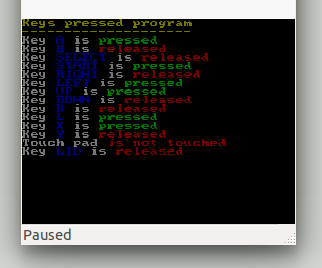
\includegraphics[scale=0.5]{p3Media/keysHeld}
    \caption{Captura del programa keysHeld.}
    \end{figure}

    \newpage

    \section{Uso avanzado del texto en pantalla}

    \subsection{custom\_font}

    En este ejemplo han creado un fichero \textbf{.bmp} que contiene por filas en una columna 95 caracteres. El programa utiliza el fichero \texttt{font.h} creado por grit y este \textbf{.bmp} para definir un variable de tipo ConsoleFont y luego lo utiliza con un \texttt{console} definido al principio del programa. Al final del programa con un simple \texttt{printf} nos muestra en el emulador la fuente custom.

    \begin{figure}[H] 
    \centering
    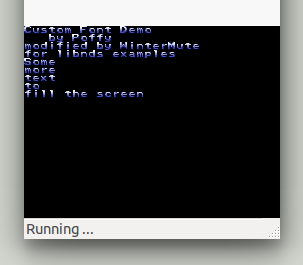
\includegraphics[scale=0.5]{p3Media/custom_font}
    \caption{Captura del programa custom\_font.}
    \end{figure}

    \newpage

    \subsection{print\_both\_screens}

    Con este programa lo que han conseguido es lanzar dos consolas simultáneamente, uno en cada pantalla de la nds. Para esto tienen que hacer uso del video mode y bancos de vram para ambas pantallas. Luego mediante la función de \texttt{consoleSelect} puede ir cambiando de consola para los \texttt{printf} que realiza. En la pantalla superior imprime un mensaje estático y en la pantalla inferior hace uso de la funcionalidad táctil mostrando en que punto se está pulsando la pantalla táctil.

    \begin{figure}[H] 
    \centering
    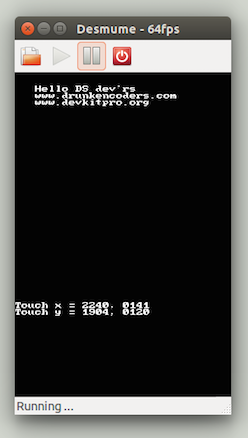
\includegraphics[scale=0.5]{p3Media/print_both_screens}
    \caption{Captura del programa print\_both\_screens.}
    \end{figure}

    \newpage

    \subsection{rotation}

    Este programa juega con una imagen puesta como fondo en la pantalla principal, mediante las teclas permite hacer varias transformaciones de la imagen con el uso de funciones de libnds. Podemos ajustar donde está centrada la imagen, el tamaño en ambas ejes y el ángulo en ambas direcciones. Por alguna razón, en el código del ejemplo, utiliza la tecla \emph{START} para cambiar el centro de la imagen en el eje x, pero también utiliza esta tecla para salir del programa. Comentando la linea que hace \texttt{break} al pulsar la tecla \emph{START} ya podemos cambiar el centro de la imagen en el eje x.

    \begin{figure}[H] 
    \centering
    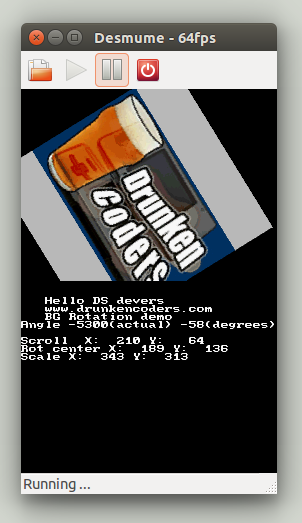
\includegraphics[scale=0.5]{p3Media/rotation}
    \caption{Captura del programa rotation.}
    \end{figure}

    \newpage

    \subsection{rotscale\_text}

    Este es muy similar al anterior, lo único que cambia es que al principio carga una fuente custom como en el ejemplo que hemos visto anteriormente y muestra la salida en la pantalla inferior. Hace las mismas operaciones sobre el fondo como en el ejemplo anterior y consigue la referencia al fondo directamente de la consola. 

    \begin{figure}[H] 
    \centering
    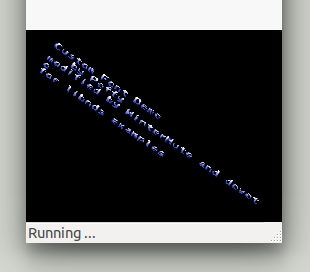
\includegraphics[scale=0.5]{p3Media/rotscale_text}
    \caption{Captura del programa rotscale\_text.}
    \end{figure}

    
    \subsection{console\_windows}

    Con el último ejemplo observamos que tenemos dos cajas en pantalla y dependiendo en que lado de la pantalla tocamos la pantalla, va escribiendo las coordinadas del toque en la caja correspondiente a esa mitad en vertical de la pantalla. Consigue esto con la función de \texttt{consoleSetWindow} variando el valor del eje x para cada una de las cajas y así imprimiendo dentro de ellas.

    \begin{figure}[H] 
    \centering
    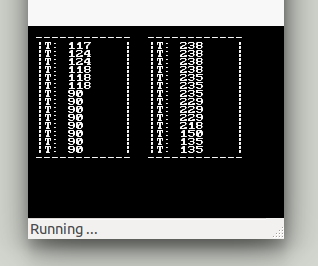
\includegraphics[scale=0.5]{p3Media/console_windows}
    \caption{Captura del programa console\_windows.}
    \end{figure}

    \newpage

    \section{Sistemas de archivos en NDS}

    \subsection{libfat}

    \texttt{fat.h}

    \textbf{Funciones:}
    \begin{enumerate}
        \item \texttt{fatInitDefault()}
        \item \texttt{opendir()}
        \item \texttt{closedir()}
        \item \texttt{readdir}
    \end{enumerate}

    \subsection{nitrofs}
      
    \texttt{filesystem.h}

    \textbf{Funciones:}
    \begin{enumerate}
        \item \texttt{nitroFSInit()}
        \item \texttt{dirlist()}
        \item \texttt{fseek}
        \item \texttt{ftell}
        \item \texttt{fread}
    \end{enumerate}


    
    
\end{document}